\documentclass[1p]{elsarticle_modified}
%\bibliographystyle{elsarticle-num}

%\usepackage[colorlinks]{hyperref}
%\usepackage{abbrmath_seonhwa} %\Abb, \Ascr, \Acal ,\Abf, \Afrak
\usepackage{amsfonts}
\usepackage{amssymb}
\usepackage{amsmath}
\usepackage{amsthm}
\usepackage{scalefnt}
\usepackage{amsbsy}
\usepackage{kotex}
\usepackage{caption}
\usepackage{subfig}
\usepackage{color}
\usepackage{graphicx}
\usepackage{xcolor} %% white, black, red, green, blue, cyan, magenta, yellow
\usepackage{float}
\usepackage{setspace}
\usepackage{hyperref}

\usepackage{tikz}
\usetikzlibrary{arrows}

\usepackage{multirow}
\usepackage{array} % fixed length table
\usepackage{hhline}

%%%%%%%%%%%%%%%%%%%%%
\makeatletter
\renewcommand*\env@matrix[1][\arraystretch]{%
	\edef\arraystretch{#1}%
	\hskip -\arraycolsep
	\let\@ifnextchar\new@ifnextchar
	\array{*\c@MaxMatrixCols c}}
\makeatother %https://tex.stackexchange.com/questions/14071/how-can-i-increase-the-line-spacing-in-a-matrix
%%%%%%%%%%%%%%%

\usepackage[normalem]{ulem}

\newcommand{\msout}[1]{\ifmmode\text{\sout{\ensuremath{#1}}}\else\sout{#1}\fi}
%SOURCE: \msout is \stkout macro in https://tex.stackexchange.com/questions/20609/strikeout-in-math-mode

\newcommand{\cancel}[1]{
	\ifmmode
	{\color{red}\msout{#1}}
	\else
	{\color{red}\sout{#1}}
	\fi
}

\newcommand{\add}[1]{
	{\color{blue}\uwave{#1}}
}

\newcommand{\replace}[2]{
	\ifmmode
	{\color{red}\msout{#1}}{\color{blue}\uwave{#2}}
	\else
	{\color{red}\sout{#1}}{\color{blue}\uwave{#2}}
	\fi
}

\newcommand{\Sol}{\mathcal{S}} %segment
\newcommand{\D}{D} %diagram
\newcommand{\A}{\mathcal{A}} %arc


%%%%%%%%%%%%%%%%%%%%%%%%%%%%%5 test

\def\sl{\operatorname{\textup{SL}}(2,\Cbb)}
\def\psl{\operatorname{\textup{PSL}}(2,\Cbb)}
\def\quan{\mkern 1mu \triangleright \mkern 1mu}

\theoremstyle{definition}
\newtheorem{thm}{Theorem}[section]
\newtheorem{prop}[thm]{Proposition}
\newtheorem{lem}[thm]{Lemma}
\newtheorem{ques}[thm]{Question}
\newtheorem{cor}[thm]{Corollary}
\newtheorem{defn}[thm]{Definition}
\newtheorem{exam}[thm]{Example}
\newtheorem{rmk}[thm]{Remark}
\newtheorem{alg}[thm]{Algorithm}

\newcommand{\I}{\sqrt{-1}}
\begin{document}

%\begin{frontmatter}
%
%\title{Boundary parabolic representations of knots up to 8 crossings}
%
%%% Group authors per affiliation:
%\author{Yunhi Cho} 
%\address{Department of Mathematics, University of Seoul, Seoul, Korea}
%\ead{yhcho@uos.ac.kr}
%
%
%\author{Seonhwa Kim} %\fnref{s_kim}}
%\address{Center for Geometry and Physics, Institute for Basic Science, Pohang, 37673, Korea}
%\ead{ryeona17@ibs.re.kr}
%
%\author{Hyuk Kim}
%\address{Department of Mathematical Sciences, Seoul National University, Seoul 08826, Korea}
%\ead{hyukkim@snu.ac.kr}
%
%\author{Seokbeom Yoon}
%\address{Department of Mathematical Sciences, Seoul National University, Seoul, 08826,  Korea}
%\ead{sbyoon15@snu.ac.kr}
%
%\begin{abstract}
%We find all boundary parabolic representation of knots up to 8 crossings.
%
%\end{abstract}
%\begin{keyword}
%    \MSC[2010] 57M25 
%\end{keyword}
%
%\end{frontmatter}

%\linenumbers
%\tableofcontents
%
\newcommand\colored[1]{\textcolor{white}{\rule[-0.35ex]{0.8em}{1.4ex}}\kern-0.8em\color{red} #1}%
%\newcommand\colored[1]{\textcolor{white}{ #1}\kern-2.17ex	\textcolor{white}{ #1}\kern-1.81ex	\textcolor{white}{ #1}\kern-2.15ex\color{red}#1	}

{\Large $\underline{12a_{0298}~(K12a_{0298})}$}

\setlength{\tabcolsep}{10pt}
\renewcommand{\arraystretch}{1.6}
\vspace{1cm}\begin{tabular}{m{100pt}>{\centering\arraybackslash}m{274pt}}
\multirow{5}{120pt}{
	\centering
	\includegraphics[width=112pt]{../../../GIT/diagram.site/Diagrams/png/1099_12a_0298.png}\\
\ \ \ A knot diagram\footnotemark}&
\allowdisplaybreaks
\textbf{Linearized knot diagam} \\
\cline{2-2}
 &
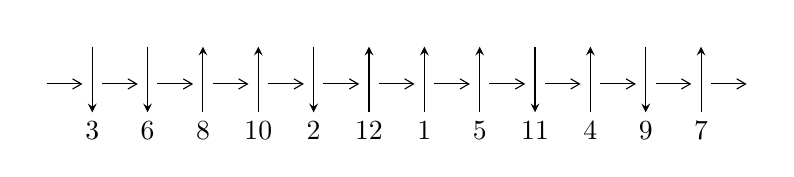
\begin{tikzpicture}[x=20pt, y=17pt]
	% nodes
	\node (C0) at (0, 0) {};
	\node (C1) at (1, 0) {};
	\node (C1U) at (1, +1) {};
	\node (C1D) at (1, -1) {3};

	\node (C2) at (2, 0) {};
	\node (C2U) at (2, +1) {};
	\node (C2D) at (2, -1) {6};

	\node (C3) at (3, 0) {};
	\node (C3U) at (3, +1) {};
	\node (C3D) at (3, -1) {8};

	\node (C4) at (4, 0) {};
	\node (C4U) at (4, +1) {};
	\node (C4D) at (4, -1) {10};

	\node (C5) at (5, 0) {};
	\node (C5U) at (5, +1) {};
	\node (C5D) at (5, -1) {2};

	\node (C6) at (6, 0) {};
	\node (C6U) at (6, +1) {};
	\node (C6D) at (6, -1) {12};

	\node (C7) at (7, 0) {};
	\node (C7U) at (7, +1) {};
	\node (C7D) at (7, -1) {1};

	\node (C8) at (8, 0) {};
	\node (C8U) at (8, +1) {};
	\node (C8D) at (8, -1) {5};

	\node (C9) at (9, 0) {};
	\node (C9U) at (9, +1) {};
	\node (C9D) at (9, -1) {11};

	\node (C10) at (10, 0) {};
	\node (C10U) at (10, +1) {};
	\node (C10D) at (10, -1) {4};

	\node (C11) at (11, 0) {};
	\node (C11U) at (11, +1) {};
	\node (C11D) at (11, -1) {9};

	\node (C12) at (12, 0) {};
	\node (C12U) at (12, +1) {};
	\node (C12D) at (12, -1) {7};
	\node (C13) at (13, 0) {};

	% arrows
	\draw[->,>={angle 60}]
	(C0) edge (C1) (C1) edge (C2) (C2) edge (C3) (C3) edge (C4) (C4) edge (C5) (C5) edge (C6) (C6) edge (C7) (C7) edge (C8) (C8) edge (C9) (C9) edge (C10) (C10) edge (C11) (C11) edge (C12) (C12) edge (C13) ;	\draw[->,>=stealth]
	(C1U) edge (C1D) (C2U) edge (C2D) (C3D) edge (C3U) (C4D) edge (C4U) (C5U) edge (C5D) (C6D) edge (C6U) (C7D) edge (C7U) (C8D) edge (C8U) (C9U) edge (C9D) (C10D) edge (C10U) (C11U) edge (C11D) (C12D) edge (C12U) ;
	\end{tikzpicture} \\
\hhline{~~} \\& 
\textbf{Solving Sequence} \\ \cline{2-2} 
 &
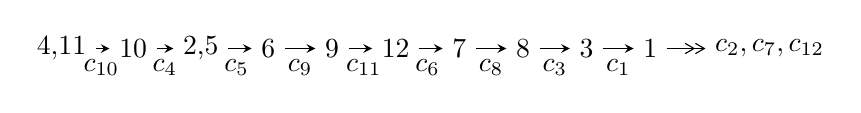
\begin{tikzpicture}[x=23pt, y=7pt]
	% node
	\node (A0) at (-1/8, 0) {4,11};
	\node (A1) at (1, 0) {10};
	\node (A2) at (33/16, 0) {2,5};
	\node (A3) at (25/8, 0) {6};
	\node (A4) at (33/8, 0) {9};
	\node (A5) at (41/8, 0) {12};
	\node (A6) at (49/8, 0) {7};
	\node (A7) at (57/8, 0) {8};
	\node (A8) at (65/8, 0) {3};
	\node (A9) at (73/8, 0) {1};
	\node (C1) at (1/2, -1) {$c_{10}$};
	\node (C2) at (3/2, -1) {$c_{4}$};
	\node (C3) at (21/8, -1) {$c_{5}$};
	\node (C4) at (29/8, -1) {$c_{9}$};
	\node (C5) at (37/8, -1) {$c_{11}$};
	\node (C6) at (45/8, -1) {$c_{6}$};
	\node (C7) at (53/8, -1) {$c_{8}$};
	\node (C8) at (61/8, -1) {$c_{3}$};
	\node (C9) at (69/8, -1) {$c_{1}$};
	\node (A10) at (11, 0) {$c_{2},c_{7},c_{12}$};

	% edge
	\draw[->,>=stealth]	
	(A0) edge (A1) (A1) edge (A2) (A2) edge (A3) (A3) edge (A4) (A4) edge (A5) (A5) edge (A6) (A6) edge (A7) (A7) edge (A8) (A8) edge (A9) ;
	\draw[->>,>={angle 60}]	
	(A9) edge (A10);
\end{tikzpicture} \\ 

\end{tabular} \\

\footnotetext{
The image of knot diagram is generated by the software ``\textbf{Draw programme}" developed by Andrew Bartholomew(\url{http://www.layer8.co.uk/maths/draw/index.htm\#Running-draw}), where we modified some parts for our purpose(\url{https://github.com/CATsTAILs/LinksPainter}).
}\phantom \\ \newline 
\centering \textbf{Ideals for irreducible components\footnotemark of $X_{\text{par}}$} 
 
\begin{align*}
I^u_{1}&=\langle 
- u^{66}-10 u^{64}+\cdots+4 b-4 u,\;- u^{66}-11 u^{64}+\cdots+4 a-2,\;u^{69}+2 u^{68}+\cdots-2 u^2+2\rangle \\
I^u_{2}&=\langle 
-412 u^8 a^2+444 u^8 a+\cdots-624 a+202,\;2 u^8 a^2- u^8 a+\cdots- a+1,\\
\phantom{I^u_{2}}&\phantom{= \langle  }u^9- u^8+2 u^7- u^6+3 u^5- u^4+2 u^3+u+1\rangle \\
I^u_{3}&=\langle 
2 u^3+u^2+b+u+1,\;u^3+2 a+3 u+2,\;u^4+u^2+2\rangle \\
I^u_{4}&=\langle 
b+u,\;a+2 u-1,\;u^2+1\rangle \\
I^u_{5}&=\langle 
- u^3- u^2+b-2 u+1,\;u^3- u^2+a- u,\;u^4+1\rangle \\
\\
I^v_{1}&=\langle 
a,\;b+1,\;v-1\rangle \\
\end{align*}
\raggedright * 6 irreducible components of $\dim_{\mathbb{C}}=0$, with total 107 representations.\\
\footnotetext{All coefficients of polynomials are rational numbers. But the coefficients are sometimes approximated in decimal forms when there is not enough margin.}
\newpage
\renewcommand{\arraystretch}{1}
\centering \section*{I. $I^u_{1}= \langle - u^{66}-10 u^{64}+\cdots+4 b-4 u,\;- u^{66}-11 u^{64}+\cdots+4 a-2,\;u^{69}+2 u^{68}+\cdots-2 u^2+2 \rangle$}
\flushleft \textbf{(i) Arc colorings}\\
\begin{tabular}{m{7pt} m{180pt} m{7pt} m{180pt} }
\flushright $a_{4}=$&$\begin{pmatrix}0\\u\end{pmatrix}$ \\
\flushright $a_{11}=$&$\begin{pmatrix}1\\0\end{pmatrix}$ \\
\flushright $a_{10}=$&$\begin{pmatrix}1\\u^2\end{pmatrix}$ \\
\flushright $a_{2}=$&$\begin{pmatrix}\frac{1}{4} u^{66}+\frac{11}{4} u^{64}+\cdots-\frac{1}{2} u+\frac{1}{2}\\\frac{1}{4} u^{66}+\frac{5}{2} u^{64}+\cdots-\frac{9}{2} u^4+u\end{pmatrix}$ \\
\flushright $a_{5}=$&$\begin{pmatrix}u\\u^3+u\end{pmatrix}$ \\
\flushright $a_{6}=$&$\begin{pmatrix}\frac{1}{2} u^{68}+\frac{11}{2} u^{66}+\cdots+u-\frac{3}{2}\\u^{68}+u^{67}+\cdots+\frac{1}{2} u+1\end{pmatrix}$ \\
\flushright $a_{9}=$&$\begin{pmatrix}u^2+1\\u^2\end{pmatrix}$ \\
\flushright $a_{12}=$&$\begin{pmatrix}u^4+u^2+1\\u^4\end{pmatrix}$ \\
\flushright $a_{7}=$&$\begin{pmatrix}-\frac{1}{4} u^{63}-\frac{5}{2} u^{61}+\cdots+\frac{1}{2} u-1\\-\frac{1}{4} u^{65}-\frac{11}{4} u^{63}+\cdots-\frac{5}{2} u^2+\frac{1}{2} u\end{pmatrix}$ \\
\flushright $a_{8}=$&$\begin{pmatrix}u^6+u^4+2 u^2+1\\u^8+2 u^6+2 u^4+2 u^2\end{pmatrix}$ \\
\flushright $a_{3}=$&$\begin{pmatrix}- u^{13}-2 u^{11}-5 u^9-6 u^7-6 u^5-4 u^3- u\\- u^{15}-3 u^{13}-6 u^{11}-9 u^9-8 u^7-6 u^5-2 u^3+u\end{pmatrix}$ \\
\flushright $a_{1}=$&$\begin{pmatrix}\frac{1}{4} u^{61}+\frac{5}{2} u^{59}+\cdots- u^2+1\\\frac{1}{4} u^{61}+\frac{9}{4} u^{59}+\cdots-\frac{1}{2} u^2+\frac{1}{2} u\end{pmatrix}$\\&\end{tabular}
\flushleft \textbf{(ii) Obstruction class $= -1$}\\~\\
\flushleft \textbf{(iii) Cusp Shapes $= 2 u^{68}+4 u^{67}+\cdots-10 u+8$}\\~\\
\newpage\renewcommand{\arraystretch}{1}
\flushleft \textbf{(iv) u-Polynomials at the component}\newline \\
\begin{tabular}{m{50pt}|m{274pt}}
Crossings & \hspace{64pt}u-Polynomials at each crossing \\
\hline $$\begin{aligned}c_{1}\end{aligned}$$&$\begin{aligned}
&u^{69}+26 u^{68}+\cdots+3481 u+256
\end{aligned}$\\
\hline $$\begin{aligned}c_{2},c_{5}\end{aligned}$$&$\begin{aligned}
&u^{69}+2 u^{68}+\cdots-5 u-16
\end{aligned}$\\
\hline $$\begin{aligned}c_{3}\end{aligned}$$&$\begin{aligned}
&u^{69}-2 u^{68}+\cdots-188076 u-54322
\end{aligned}$\\
\hline $$\begin{aligned}c_{4},c_{10}\end{aligned}$$&$\begin{aligned}
&u^{69}-2 u^{68}+\cdots+2 u^2-2
\end{aligned}$\\
\hline $$\begin{aligned}c_{6},c_{7},c_{12}\end{aligned}$$&$\begin{aligned}
&u^{69}-2 u^{68}+\cdots-37 u-16
\end{aligned}$\\
\hline $$\begin{aligned}c_{8}\end{aligned}$$&$\begin{aligned}
&u^{69}+10 u^{68}+\cdots-2116 u-86
\end{aligned}$\\
\hline $$\begin{aligned}c_{9},c_{11}\end{aligned}$$&$\begin{aligned}
&u^{69}+22 u^{68}+\cdots+8 u-4
\end{aligned}$\\
\hline
\end{tabular}\\~\\
\newpage\renewcommand{\arraystretch}{1}
\flushleft \textbf{(v) Riley Polynomials at the component}\newline \\
\begin{tabular}{m{50pt}|m{274pt}}
Crossings & \hspace{64pt}Riley Polynomials at each crossing \\
\hline $$\begin{aligned}c_{1}\end{aligned}$$&$\begin{aligned}
&y^{69}+46 y^{68}+\cdots-2589327 y-65536
\end{aligned}$\\
\hline $$\begin{aligned}c_{2},c_{5}\end{aligned}$$&$\begin{aligned}
&y^{69}-26 y^{68}+\cdots+3481 y-256
\end{aligned}$\\
\hline $$\begin{aligned}c_{3}\end{aligned}$$&$\begin{aligned}
&y^{69}-26 y^{68}+\cdots+15690417448 y-2950879684
\end{aligned}$\\
\hline $$\begin{aligned}c_{4},c_{10}\end{aligned}$$&$\begin{aligned}
&y^{69}+22 y^{68}+\cdots+8 y-4
\end{aligned}$\\
\hline $$\begin{aligned}c_{6},c_{7},c_{12}\end{aligned}$$&$\begin{aligned}
&y^{69}-74 y^{68}+\cdots-10919 y-256
\end{aligned}$\\
\hline $$\begin{aligned}c_{8}\end{aligned}$$&$\begin{aligned}
&y^{69}-2 y^{68}+\cdots-1189944 y-7396
\end{aligned}$\\
\hline $$\begin{aligned}c_{9},c_{11}\end{aligned}$$&$\begin{aligned}
&y^{69}+50 y^{68}+\cdots+768 y-16
\end{aligned}$\\
\hline
\end{tabular}\\~\\
\newpage\flushleft \textbf{(vi) Complex Volumes and Cusp Shapes}
$$\begin{array}{c|c|c}  
\text{Solutions to }I^u_{1}& \I (\text{vol} + \sqrt{-1}CS) & \text{Cusp shape}\\
 \hline 
\begin{aligned}
u &= -0.735899 + 0.688576 I \\
a &= -1.41058 - 0.11854 I \\
b &= -0.96277 + 2.11478 I\end{aligned}
 & -0.240515 + 0.033439 I & -1.48136 + 0. I\phantom{ +0.000000I} \\ \hline\begin{aligned}
u &= -0.735899 - 0.688576 I \\
a &= -1.41058 + 0.11854 I \\
b &= -0.96277 - 2.11478 I\end{aligned}
 & -0.240515 - 0.033439 I & -1.48136 + 0. I\phantom{ +0.000000I} \\ \hline\begin{aligned}
u &= \phantom{-}0.338664 + 0.953969 I \\
a &= \phantom{-}0.259722 + 0.602753 I \\
b &= \phantom{-}0.242668 + 1.080750 I\end{aligned}
 & \phantom{-}5.18981 + 0.99757 I & \phantom{-}4.76342 - 3.46084 I \\ \hline\begin{aligned}
u &= \phantom{-}0.338664 - 0.953969 I \\
a &= \phantom{-}0.259722 - 0.602753 I \\
b &= \phantom{-}0.242668 - 1.080750 I\end{aligned}
 & \phantom{-}5.18981 - 0.99757 I & \phantom{-}4.76342 + 3.46084 I \\ \hline\begin{aligned}
u &= \phantom{-}0.484849 + 0.860276 I \\
a &= \phantom{-}1.27015 + 0.75092 I \\
b &= -0.89181 + 2.10893 I\end{aligned}
 & -1.85693 - 1.13119 I & -2.07731 + 1.47337 I \\ \hline\begin{aligned}
u &= \phantom{-}0.484849 - 0.860276 I \\
a &= \phantom{-}1.27015 - 0.75092 I \\
b &= -0.89181 - 2.10893 I\end{aligned}
 & -1.85693 + 1.13119 I & -2.07731 - 1.47337 I \\ \hline\begin{aligned}
u &= \phantom{-}0.058334 + 1.021690 I \\
a &= \phantom{-}0.24060 - 2.11026 I \\
b &= \phantom{-}0.529272 - 0.918124 I\end{aligned}
 & -5.74447 - 0.01900 I & -8.65927 + 0. I\phantom{ +0.000000I} \\ \hline\begin{aligned}
u &= \phantom{-}0.058334 - 1.021690 I \\
a &= \phantom{-}0.24060 + 2.11026 I \\
b &= \phantom{-}0.529272 + 0.918124 I\end{aligned}
 & -5.74447 + 0.01900 I & -8.65927 + 0. I\phantom{ +0.000000I} \\ \hline\begin{aligned}
u &= \phantom{-}0.154964 + 1.031240 I \\
a &= -0.85296 + 1.99168 I \\
b &= -0.216276 + 0.724886 I\end{aligned}
 & -3.54966 + 6.72812 I & -3.30535 - 7.86468 I \\ \hline\begin{aligned}
u &= \phantom{-}0.154964 - 1.031240 I \\
a &= -0.85296 - 1.99168 I \\
b &= -0.216276 - 0.724886 I\end{aligned}
 & -3.54966 - 6.72812 I & -3.30535 + 7.86468 I\\
 \hline 
 \end{array}$$\newpage$$\begin{array}{c|c|c}  
\text{Solutions to }I^u_{1}& \I (\text{vol} + \sqrt{-1}CS) & \text{Cusp shape}\\
 \hline 
\begin{aligned}
u &= \phantom{-}0.718154 + 0.761613 I \\
a &= \phantom{-}0.040869 + 0.875751 I \\
b &= -0.531478 + 0.949465 I\end{aligned}
 & \phantom{-}3.60394 - 0.19911 I & \phantom{-}9.90804 + 0. I\phantom{ +0.000000I} \\ \hline\begin{aligned}
u &= \phantom{-}0.718154 - 0.761613 I \\
a &= \phantom{-}0.040869 - 0.875751 I \\
b &= -0.531478 - 0.949465 I\end{aligned}
 & \phantom{-}3.60394 + 0.19911 I & \phantom{-}9.90804 + 0. I\phantom{ +0.000000I} \\ \hline\begin{aligned}
u &= -0.422383 + 0.968673 I \\
a &= -0.599532 + 1.252790 I \\
b &= \phantom{-}1.85369 + 1.47586 I\end{aligned}
 & \phantom{-}3.61056 + 4.51985 I & \phantom{-0.000000 } 0 \\ \hline\begin{aligned}
u &= -0.422383 - 0.968673 I \\
a &= -0.599532 - 1.252790 I \\
b &= \phantom{-}1.85369 - 1.47586 I\end{aligned}
 & \phantom{-}3.61056 - 4.51985 I & \phantom{-0.000000 } 0 \\ \hline\begin{aligned}
u &= \phantom{-}0.193872 + 1.039360 I \\
a &= -0.624526 + 0.079575 I \\
b &= -0.927525 - 0.005005 I\end{aligned}
 & \phantom{-}4.24263 + 5.04361 I & \phantom{-0.000000 } 0. - 4.03426 I \\ \hline\begin{aligned}
u &= \phantom{-}0.193872 - 1.039360 I \\
a &= -0.624526 - 0.079575 I \\
b &= -0.927525 + 0.005005 I\end{aligned}
 & \phantom{-}4.24263 - 5.04361 I & \phantom{-0.000000 -}0. + 4.03426 I \\ \hline\begin{aligned}
u &= \phantom{-}0.721986 + 0.582383 I \\
a &= \phantom{-}1.020400 - 0.497911 I \\
b &= \phantom{-}1.35891 + 1.25471 I\end{aligned}
 & \phantom{-}3.90829 + 1.18050 I & \phantom{-}7.40920 - 3.02522 I \\ \hline\begin{aligned}
u &= \phantom{-}0.721986 - 0.582383 I \\
a &= \phantom{-}1.020400 + 0.497911 I \\
b &= \phantom{-}1.35891 - 1.25471 I\end{aligned}
 & \phantom{-}3.90829 - 1.18050 I & \phantom{-}7.40920 + 3.02522 I \\ \hline\begin{aligned}
u &= -0.814686 + 0.705728 I \\
a &= \phantom{-}2.39011 + 0.79666 I \\
b &= \phantom{-}2.59506 - 2.01293 I\end{aligned}
 & \phantom{-}2.93810 + 6.44249 I & \phantom{-0.000000 } 0 \\ \hline\begin{aligned}
u &= -0.814686 - 0.705728 I \\
a &= \phantom{-}2.39011 - 0.79666 I \\
b &= \phantom{-}2.59506 + 2.01293 I\end{aligned}
 & \phantom{-}2.93810 - 6.44249 I & \phantom{-0.000000 } 0\\
 \hline 
 \end{array}$$\newpage$$\begin{array}{c|c|c}  
\text{Solutions to }I^u_{1}& \I (\text{vol} + \sqrt{-1}CS) & \text{Cusp shape}\\
 \hline 
\begin{aligned}
u &= -0.028573 + 1.077810 I \\
a &= -0.61215 - 1.87207 I \\
b &= -0.511359 - 0.452462 I\end{aligned}
 & -1.60521 + 2.06429 I & \phantom{-0.000000 } 0 \\ \hline\begin{aligned}
u &= -0.028573 - 1.077810 I \\
a &= -0.61215 + 1.87207 I \\
b &= -0.511359 + 0.452462 I\end{aligned}
 & -1.60521 - 2.06429 I & \phantom{-0.000000 } 0 \\ \hline\begin{aligned}
u &= -0.170360 + 1.066470 I \\
a &= \phantom{-}0.37501 + 2.28994 I \\
b &= \phantom{-}0.350653 + 0.759401 I\end{aligned}
 & \phantom{-}2.10642 - 10.83270 I & \phantom{-0.000000 -}0. + 7.91871 I \\ \hline\begin{aligned}
u &= -0.170360 - 1.066470 I \\
a &= \phantom{-}0.37501 - 2.28994 I \\
b &= \phantom{-}0.350653 - 0.759401 I\end{aligned}
 & \phantom{-}2.10642 + 10.83270 I & \phantom{-0.000000 } 0. - 7.91871 I \\ \hline\begin{aligned}
u &= \phantom{-}0.836381 + 0.694622 I \\
a &= -2.53666 + 0.36324 I \\
b &= -2.27305 - 2.69677 I\end{aligned}
 & \phantom{-}8.89008 - 10.76610 I & \phantom{-0.000000 } 0 \\ \hline\begin{aligned}
u &= \phantom{-}0.836381 - 0.694622 I \\
a &= -2.53666 - 0.36324 I \\
b &= -2.27305 + 2.69677 I\end{aligned}
 & \phantom{-}8.89008 + 10.76610 I & \phantom{-0.000000 } 0 \\ \hline\begin{aligned}
u &= -0.833721 + 0.715169 I \\
a &= -0.612597 + 0.721125 I \\
b &= \phantom{-}0.402951 + 0.631456 I\end{aligned}
 & \phantom{-}11.06750 + 4.64835 I & \phantom{-0.000000 } 0 \\ \hline\begin{aligned}
u &= -0.833721 - 0.715169 I \\
a &= -0.612597 - 0.721125 I \\
b &= \phantom{-}0.402951 - 0.631456 I\end{aligned}
 & \phantom{-}11.06750 - 4.64835 I & \phantom{-0.000000 } 0 \\ \hline\begin{aligned}
u &= -0.788117 + 0.777559 I \\
a &= -0.860399 - 0.145200 I \\
b &= -1.208460 - 0.042361 I\end{aligned}
 & \phantom{-}4.23303 - 3.52292 I & \phantom{-0.000000 } 0 \\ \hline\begin{aligned}
u &= -0.788117 - 0.777559 I \\
a &= -0.860399 + 0.145200 I \\
b &= -1.208460 + 0.042361 I\end{aligned}
 & \phantom{-}4.23303 + 3.52292 I & \phantom{-0.000000 } 0\\
 \hline 
 \end{array}$$\newpage$$\begin{array}{c|c|c}  
\text{Solutions to }I^u_{1}& \I (\text{vol} + \sqrt{-1}CS) & \text{Cusp shape}\\
 \hline 
\begin{aligned}
u &= -0.821959 + 0.782703 I \\
a &= \phantom{-}1.141410 + 0.345243 I \\
b &= \phantom{-}0.680996 - 0.881071 I\end{aligned}
 & \phantom{-}12.26590 - 0.79570 I & \phantom{-0.000000 } 0 \\ \hline\begin{aligned}
u &= -0.821959 - 0.782703 I \\
a &= \phantom{-}1.141410 - 0.345243 I \\
b &= \phantom{-}0.680996 + 0.881071 I\end{aligned}
 & \phantom{-}12.26590 + 0.79570 I & \phantom{-0.000000 } 0 \\ \hline\begin{aligned}
u &= \phantom{-}0.611116 + 0.956461 I \\
a &= -0.49978 - 2.05095 I \\
b &= \phantom{-}2.42886 - 2.48221 I\end{aligned}
 & -2.54832 + 5.58402 I & \phantom{-0.000000 } 0 \\ \hline\begin{aligned}
u &= \phantom{-}0.611116 - 0.956461 I \\
a &= -0.49978 + 2.05095 I \\
b &= \phantom{-}2.42886 + 2.48221 I\end{aligned}
 & -2.54832 - 5.58402 I & \phantom{-0.000000 } 0 \\ \hline\begin{aligned}
u &= \phantom{-}0.814707 + 0.809092 I \\
a &= \phantom{-}0.295475 - 0.322981 I \\
b &= \phantom{-}0.913082 - 1.062150 I\end{aligned}
 & \phantom{-}10.93290 + 7.02859 I & \phantom{-0.000000 } 0 \\ \hline\begin{aligned}
u &= \phantom{-}0.814707 - 0.809092 I \\
a &= \phantom{-}0.295475 + 0.322981 I \\
b &= \phantom{-}0.913082 + 1.062150 I\end{aligned}
 & \phantom{-}10.93290 - 7.02859 I & \phantom{-0.000000 } 0 \\ \hline\begin{aligned}
u &= \phantom{-}0.695607 + 0.941949 I \\
a &= -0.886074 - 0.080146 I \\
b &= -0.262992 - 0.787216 I\end{aligned}
 & \phantom{-}3.05990 + 5.61567 I & \phantom{-0.000000 } 0 \\ \hline\begin{aligned}
u &= \phantom{-}0.695607 - 0.941949 I \\
a &= -0.886074 + 0.080146 I \\
b &= -0.262992 + 0.787216 I\end{aligned}
 & \phantom{-}3.05990 - 5.61567 I & \phantom{-0.000000 } 0 \\ \hline\begin{aligned}
u &= -0.044024 + 0.818063 I \\
a &= \phantom{-}0.652335 - 0.322162 I \\
b &= -0.167905 + 0.623453 I\end{aligned}
 & -1.27770 - 1.44146 I & \phantom{-}0.19549 + 5.54807 I \\ \hline\begin{aligned}
u &= -0.044024 - 0.818063 I \\
a &= \phantom{-}0.652335 + 0.322162 I \\
b &= -0.167905 - 0.623453 I\end{aligned}
 & -1.27770 + 1.44146 I & \phantom{-}0.19549 - 5.54807 I\\
 \hline 
 \end{array}$$\newpage$$\begin{array}{c|c|c}  
\text{Solutions to }I^u_{1}& \I (\text{vol} + \sqrt{-1}CS) & \text{Cusp shape}\\
 \hline 
\begin{aligned}
u &= -0.613808 + 1.009340 I \\
a &= \phantom{-}0.84248 - 1.87193 I \\
b &= -2.04716 - 2.64513 I\end{aligned}
 & \phantom{-}1.96131 - 8.32605 I & \phantom{-0.000000 } 0 \\ \hline\begin{aligned}
u &= -0.613808 - 1.009340 I \\
a &= \phantom{-}0.84248 + 1.87193 I \\
b &= -2.04716 + 2.64513 I\end{aligned}
 & \phantom{-}1.96131 + 8.32605 I & \phantom{-0.000000 } 0 \\ \hline\begin{aligned}
u &= -0.662707 + 0.477450 I \\
a &= -1.86190 + 0.54426 I \\
b &= -0.57360 + 1.90850 I\end{aligned}
 & \phantom{-}3.39108 + 3.42806 I & \phantom{-}6.35256 - 3.02642 I \\ \hline\begin{aligned}
u &= -0.662707 - 0.477450 I \\
a &= -1.86190 - 0.54426 I \\
b &= -0.57360 - 1.90850 I\end{aligned}
 & \phantom{-}3.39108 - 3.42806 I & \phantom{-}6.35256 + 3.02642 I \\ \hline\begin{aligned}
u &= -0.737691 + 0.955567 I \\
a &= -0.388118 - 0.820537 I \\
b &= -0.573332 + 0.251331 I\end{aligned}
 & \phantom{-}3.68498 - 2.23055 I & \phantom{-0.000000 } 0 \\ \hline\begin{aligned}
u &= -0.737691 - 0.955567 I \\
a &= -0.388118 + 0.820537 I \\
b &= -0.573332 - 0.251331 I\end{aligned}
 & \phantom{-}3.68498 + 2.23055 I & \phantom{-0.000000 } 0 \\ \hline\begin{aligned}
u &= -0.689892 + 0.991018 I \\
a &= \phantom{-}0.09117 - 1.66872 I \\
b &= -2.85026 - 1.61053 I\end{aligned}
 & -1.14588 - 5.49156 I & \phantom{-0.000000 } 0 \\ \hline\begin{aligned}
u &= -0.689892 - 0.991018 I \\
a &= \phantom{-}0.09117 + 1.66872 I \\
b &= -2.85026 + 1.61053 I\end{aligned}
 & -1.14588 + 5.49156 I & \phantom{-0.000000 } 0 \\ \hline\begin{aligned}
u &= \phantom{-}0.659252 + 1.016190 I \\
a &= \phantom{-}0.137976 - 1.363260 I \\
b &= \phantom{-}2.56392 - 0.66959 I\end{aligned}
 & \phantom{-}2.66779 + 4.10740 I & \phantom{-0.000000 } 0 \\ \hline\begin{aligned}
u &= \phantom{-}0.659252 - 1.016190 I \\
a &= \phantom{-}0.137976 + 1.363260 I \\
b &= \phantom{-}2.56392 + 0.66959 I\end{aligned}
 & \phantom{-}2.66779 - 4.10740 I & \phantom{-0.000000 } 0\\
 \hline 
 \end{array}$$\newpage$$\begin{array}{c|c|c}  
\text{Solutions to }I^u_{1}& \I (\text{vol} + \sqrt{-1}CS) & \text{Cusp shape}\\
 \hline 
\begin{aligned}
u &= \phantom{-}0.771414 + 0.943358 I \\
a &= \phantom{-}0.552899 - 0.216552 I \\
b &= -0.327428 + 0.913552 I\end{aligned}
 & \phantom{-}10.51840 - 1.09087 I & \phantom{-0.000000 } 0 \\ \hline\begin{aligned}
u &= \phantom{-}0.771414 - 0.943358 I \\
a &= \phantom{-}0.552899 + 0.216552 I \\
b &= -0.327428 - 0.913552 I\end{aligned}
 & \phantom{-}10.51840 + 1.09087 I & \phantom{-0.000000 } 0 \\ \hline\begin{aligned}
u &= -0.764178 + 0.965173 I \\
a &= \phantom{-}0.412858 + 1.010290 I \\
b &= \phantom{-}1.49440 + 0.94058 I\end{aligned}
 & \phantom{-}11.70390 - 5.14096 I & \phantom{-0.000000 } 0 \\ \hline\begin{aligned}
u &= -0.764178 - 0.965173 I \\
a &= \phantom{-}0.412858 - 1.010290 I \\
b &= \phantom{-}1.49440 - 0.94058 I\end{aligned}
 & \phantom{-}11.70390 + 5.14096 I & \phantom{-0.000000 } 0 \\ \hline\begin{aligned}
u &= -0.729127 + 1.006320 I \\
a &= \phantom{-}0.85456 + 2.40770 I \\
b &= \phantom{-}4.06882 + 0.97788 I\end{aligned}
 & \phantom{-}2.02182 - 12.24190 I & \phantom{-0.000000 } 0 \\ \hline\begin{aligned}
u &= -0.729127 - 1.006320 I \\
a &= \phantom{-}0.85456 - 2.40770 I \\
b &= \phantom{-}4.06882 - 0.97788 I\end{aligned}
 & \phantom{-}2.02182 + 12.24190 I & \phantom{-0.000000 } 0 \\ \hline\begin{aligned}
u &= -0.741771 + 1.008840 I \\
a &= \phantom{-}0.545247 - 0.543242 I \\
b &= \phantom{-}0.321004 - 1.292670 I\end{aligned}
 & \phantom{-}10.1674 - 10.5435 I & \phantom{-0.000000 } 0 \\ \hline\begin{aligned}
u &= -0.741771 - 1.008840 I \\
a &= \phantom{-}0.545247 + 0.543242 I \\
b &= \phantom{-}0.321004 + 1.292670 I\end{aligned}
 & \phantom{-}10.1674 + 10.5435 I & \phantom{-0.000000 } 0 \\ \hline\begin{aligned}
u &= \phantom{-}0.734769 + 1.019640 I \\
a &= -0.36453 + 2.55787 I \\
b &= -4.11635 + 1.81421 I\end{aligned}
 & \phantom{-}7.8960 + 16.6434 I & \phantom{-0.000000 } 0 \\ \hline\begin{aligned}
u &= \phantom{-}0.734769 - 1.019640 I \\
a &= -0.36453 - 2.55787 I \\
b &= -4.11635 - 1.81421 I\end{aligned}
 & \phantom{-}7.8960 - 16.6434 I & \phantom{-0.000000 } 0\\
 \hline 
 \end{array}$$\newpage$$\begin{array}{c|c|c}  
\text{Solutions to }I^u_{1}& \I (\text{vol} + \sqrt{-1}CS) & \text{Cusp shape}\\
 \hline 
\begin{aligned}
u &= -0.670400 + 0.147828 I \\
a &= \phantom{-}1.80229 + 0.50503 I \\
b &= \phantom{-}1.30651 - 0.96838 I\end{aligned}
 & \phantom{-}6.05766 - 8.22168 I & \phantom{-}7.69702 + 5.92932 I \\ \hline\begin{aligned}
u &= -0.670400 - 0.147828 I \\
a &= \phantom{-}1.80229 - 0.50503 I \\
b &= \phantom{-}1.30651 + 0.96838 I\end{aligned}
 & \phantom{-}6.05766 + 8.22168 I & \phantom{-}7.69702 - 5.92932 I \\ \hline\begin{aligned}
u &= \phantom{-}0.656891 + 0.088355 I \\
a &= -0.868107 - 1.024770 I \\
b &= -0.163464 - 0.301668 I\end{aligned}
 & \phantom{-}7.87968 + 2.33195 I & \phantom{-}10.31373 - 1.18340 I \\ \hline\begin{aligned}
u &= \phantom{-}0.656891 - 0.088355 I \\
a &= -0.868107 + 1.024770 I \\
b &= -0.163464 + 0.301668 I\end{aligned}
 & \phantom{-}7.87968 - 2.33195 I & \phantom{-}10.31373 + 1.18340 I \\ \hline\begin{aligned}
u &= \phantom{-}0.412551 + 0.453150 I \\
a &= \phantom{-}1.75896 - 0.29485 I \\
b &= \phantom{-}0.385319 + 1.182700 I\end{aligned}
 & -1.61119 - 1.13122 I & -1.25895 + 1.21665 I \\ \hline\begin{aligned}
u &= \phantom{-}0.412551 - 0.453150 I \\
a &= \phantom{-}1.75896 + 0.29485 I \\
b &= \phantom{-}0.385319 - 1.182700 I\end{aligned}
 & -1.61119 + 1.13122 I & -1.25895 - 1.21665 I \\ \hline\begin{aligned}
u &= \phantom{-}0.591730 + 0.129745 I \\
a &= -1.49243 + 0.30843 I \\
b &= -0.650903 - 1.070410 I\end{aligned}
 & \phantom{-}0.12986 + 4.40376 I & \phantom{-}4.64576 - 6.38172 I \\ \hline\begin{aligned}
u &= \phantom{-}0.591730 - 0.129745 I \\
a &= -1.49243 - 0.30843 I \\
b &= -0.650903 + 1.070410 I\end{aligned}
 & \phantom{-}0.12986 - 4.40376 I & \phantom{-}4.64576 + 6.38172 I \\ \hline\begin{aligned}
u &= -0.371894\phantom{ +0.000000I} \\
a &= \phantom{-}0.571634\phantom{ +0.000000I} \\
b &= -0.480013\phantom{ +0.000000I}\end{aligned}
 & \phantom{-}0.931539\phantom{ +0.000000I} & \phantom{-}11.9680\phantom{ +0.000000I}\\
 \hline 
 \end{array}$$\newpage\newpage\renewcommand{\arraystretch}{1}
\centering \section*{II. $I^u_{2}= \langle -412 u^8 a^2+444 u^8 a+\cdots-624 a+202,\;2 u^8 a^2- u^8 a+\cdots- a+1,\;u^9- u^8+2 u^7- u^6+3 u^5- u^4+2 u^3+u+1 \rangle$}
\flushleft \textbf{(i) Arc colorings}\\
\begin{tabular}{m{7pt} m{180pt} m{7pt} m{180pt} }
\flushright $a_{4}=$&$\begin{pmatrix}0\\u\end{pmatrix}$ \\
\flushright $a_{11}=$&$\begin{pmatrix}1\\0\end{pmatrix}$ \\
\flushright $a_{10}=$&$\begin{pmatrix}1\\u^2\end{pmatrix}$ \\
\flushright $a_{2}=$&$\begin{pmatrix}a\\0.235026 a^{2} u^{8}-0.253280 a u^{8}+\cdots+0.355961 a-0.115231\end{pmatrix}$ \\
\flushright $a_{5}=$&$\begin{pmatrix}u\\u^3+u\end{pmatrix}$ \\
\flushright $a_{6}=$&$\begin{pmatrix}1.13862 a^{2} u^{8}+0.287507 a u^{8}+\cdots+0.190531 a-0.247576\\0.854535 a^{2} u^{8}+1.25385 a u^{8}+\cdots-1.11352 a+0.309184\end{pmatrix}$ \\
\flushright $a_{9}=$&$\begin{pmatrix}u^2+1\\u^2\end{pmatrix}$ \\
\flushright $a_{12}=$&$\begin{pmatrix}u^4+u^2+1\\u^4\end{pmatrix}$ \\
\flushright $a_{7}=$&$\begin{pmatrix}0.983457 a^{2} u^{8}-0.108386 a u^{8}+\cdots-0.0638905 a-0.851112\\0.826013 a^{2} u^{8}+1.34284 a u^{8}+\cdots-1.29264 a+0.565887\end{pmatrix}$ \\
\flushright $a_{8}=$&$\begin{pmatrix}u^6+u^4+2 u^2+1\\u^8+2 u^6+2 u^4+2 u^2\end{pmatrix}$ \\
\flushright $a_{3}=$&$\begin{pmatrix}u^4+u^2+1\\u^4\end{pmatrix}$ \\
\flushright $a_{1}=$&$\begin{pmatrix}-0.142042 a^{2} u^{8}+0.483172 a u^{8}+\cdots-0.652025 a+0.278380\\0.157444 a^{2} u^{8}-0.451226 a u^{8}+\cdots-0.771249 a-1.41700\end{pmatrix}$\\&\end{tabular}
\flushleft \textbf{(ii) Obstruction class $= -1$}\\~\\
\flushleft \textbf{(iii) Cusp Shapes $= -4 u^7+4 u^6-4 u^5+4 u^4-8 u^3+4 u^2+6$}\\~\\
\newpage\renewcommand{\arraystretch}{1}
\flushleft \textbf{(iv) u-Polynomials at the component}\newline \\
\begin{tabular}{m{50pt}|m{274pt}}
Crossings & \hspace{64pt}u-Polynomials at each crossing \\
\hline $$\begin{aligned}c_{1}\end{aligned}$$&$\begin{aligned}
&u^{27}+18 u^{26}+\cdots+u+1
\end{aligned}$\\
\hline $$\begin{aligned}c_{2},c_{5},c_{6}\\c_{7},c_{12}\end{aligned}$$&$\begin{aligned}
&u^{27}-9 u^{25}+\cdots+u+1
\end{aligned}$\\
\hline $$\begin{aligned}c_{3}\end{aligned}$$&$\begin{aligned}
&(u^9+u^8-2 u^7-3 u^6+u^5+3 u^4+2 u^3- u-1)^3
\end{aligned}$\\
\hline $$\begin{aligned}c_{4},c_{10}\end{aligned}$$&$\begin{aligned}
&(u^9+u^8+2 u^7+u^6+3 u^5+u^4+2 u^3+u-1)^3
\end{aligned}$\\
\hline $$\begin{aligned}c_{8}\end{aligned}$$&$\begin{aligned}
&(u^9-5 u^8+12 u^7-15 u^6+9 u^5+u^4-4 u^3+2 u^2+u-1)^3
\end{aligned}$\\
\hline $$\begin{aligned}c_{9},c_{11}\end{aligned}$$&$\begin{aligned}
&(u^9+3 u^8+8 u^7+13 u^6+17 u^5+17 u^4+12 u^3+6 u^2+u-1)^3
\end{aligned}$\\
\hline
\end{tabular}\\~\\
\newpage\renewcommand{\arraystretch}{1}
\flushleft \textbf{(v) Riley Polynomials at the component}\newline \\
\begin{tabular}{m{50pt}|m{274pt}}
Crossings & \hspace{64pt}Riley Polynomials at each crossing \\
\hline $$\begin{aligned}c_{1}\end{aligned}$$&$\begin{aligned}
&y^{27}-18 y^{26}+\cdots+y-1
\end{aligned}$\\
\hline $$\begin{aligned}c_{2},c_{5},c_{6}\\c_{7},c_{12}\end{aligned}$$&$\begin{aligned}
&y^{27}-18 y^{26}+\cdots+y-1
\end{aligned}$\\
\hline $$\begin{aligned}c_{3}\end{aligned}$$&$\begin{aligned}
&(y^9-5 y^8+12 y^7-15 y^6+9 y^5+y^4-4 y^3+2 y^2+y-1)^3
\end{aligned}$\\
\hline $$\begin{aligned}c_{4},c_{10}\end{aligned}$$&$\begin{aligned}
&(y^9+3 y^8+8 y^7+13 y^6+17 y^5+17 y^4+12 y^3+6 y^2+y-1)^3
\end{aligned}$\\
\hline $$\begin{aligned}c_{8}\end{aligned}$$&$\begin{aligned}
&(y^9- y^8+12 y^7-7 y^6+37 y^5+y^4-10 y^2+5 y-1)^3
\end{aligned}$\\
\hline $$\begin{aligned}c_{9},c_{11}\end{aligned}$$&$\begin{aligned}
&(y^9+7 y^8+20 y^7+25 y^6+5 y^5-15 y^4+22 y^2+13 y-1)^3
\end{aligned}$\\
\hline
\end{tabular}\\~\\
\newpage\flushleft \textbf{(vi) Complex Volumes and Cusp Shapes}
$$\begin{array}{c|c|c}  
\text{Solutions to }I^u_{2}& \I (\text{vol} + \sqrt{-1}CS) & \text{Cusp shape}\\
 \hline 
\begin{aligned}
u &= -0.140343 + 0.966856 I \\
a &= \phantom{-}1.25673 + 1.05313 I \\
b &= \phantom{-}0.049646 + 0.706168 I\end{aligned}
 & -1.78344 - 2.09337 I & -0.51499 + 4.16283 I \\ \hline\begin{aligned}
u &= -0.140343 + 0.966856 I \\
a &= \phantom{-}0.163898 - 0.278866 I \\
b &= \phantom{-}0.601292 + 0.256808 I\end{aligned}
 & -1.78344 - 2.09337 I & -0.51499 + 4.16283 I \\ \hline\begin{aligned}
u &= -0.140343 + 0.966856 I \\
a &= -0.01736 - 2.34952 I \\
b &= -0.95932 - 1.47752 I\end{aligned}
 & -1.78344 - 2.09337 I & -0.51499 + 4.16283 I \\ \hline\begin{aligned}
u &= -0.140343 - 0.966856 I \\
a &= \phantom{-}1.25673 - 1.05313 I \\
b &= \phantom{-}0.049646 - 0.706168 I\end{aligned}
 & -1.78344 + 2.09337 I & -0.51499 - 4.16283 I \\ \hline\begin{aligned}
u &= -0.140343 - 0.966856 I \\
a &= \phantom{-}0.163898 + 0.278866 I \\
b &= \phantom{-}0.601292 - 0.256808 I\end{aligned}
 & -1.78344 + 2.09337 I & -0.51499 - 4.16283 I \\ \hline\begin{aligned}
u &= -0.140343 - 0.966856 I \\
a &= -0.01736 + 2.34952 I \\
b &= -0.95932 + 1.47752 I\end{aligned}
 & -1.78344 + 2.09337 I & -0.51499 - 4.16283 I \\ \hline\begin{aligned}
u &= -0.628449 + 0.875112 I \\
a &= \phantom{-}0.0738554 + 0.0112823 I \\
b &= -0.329184 + 0.287114 I\end{aligned}
 & \phantom{-}0.61694 - 2.45442 I & \phantom{-}2.32792 + 2.91298 I \\ \hline\begin{aligned}
u &= -0.628449 + 0.875112 I \\
a &= -2.10033 + 0.25220 I \\
b &= -0.22682 + 3.11202 I\end{aligned}
 & \phantom{-}0.61694 - 2.45442 I & \phantom{-}2.32792 + 2.91298 I \\ \hline\begin{aligned}
u &= -0.628449 + 0.875112 I \\
a &= \phantom{-}0.05733 - 2.33941 I \\
b &= -2.96621 - 2.53925 I\end{aligned}
 & \phantom{-}0.61694 - 2.45442 I & \phantom{-}2.32792 + 2.91298 I \\ \hline\begin{aligned}
u &= -0.628449 - 0.875112 I \\
a &= \phantom{-}0.0738554 - 0.0112823 I \\
b &= -0.329184 - 0.287114 I\end{aligned}
 & \phantom{-}0.61694 + 2.45442 I & \phantom{-}2.32792 - 2.91298 I\\
 \hline 
 \end{array}$$\newpage$$\begin{array}{c|c|c}  
\text{Solutions to }I^u_{2}& \I (\text{vol} + \sqrt{-1}CS) & \text{Cusp shape}\\
 \hline 
\begin{aligned}
u &= -0.628449 - 0.875112 I \\
a &= -2.10033 - 0.25220 I \\
b &= -0.22682 - 3.11202 I\end{aligned}
 & \phantom{-}0.61694 + 2.45442 I & \phantom{-}2.32792 - 2.91298 I \\ \hline\begin{aligned}
u &= -0.628449 - 0.875112 I \\
a &= \phantom{-}0.05733 + 2.33941 I \\
b &= -2.96621 + 2.53925 I\end{aligned}
 & \phantom{-}0.61694 + 2.45442 I & \phantom{-}2.32792 - 2.91298 I \\ \hline\begin{aligned}
u &= \phantom{-}0.796005 + 0.733148 I \\
a &= \phantom{-}0.897099 + 0.478488 I \\
b &= \phantom{-}0.366734 + 0.756648 I\end{aligned}
 & \phantom{-}4.37135 - 1.33617 I & \phantom{-}7.28409 + 0.70175 I \\ \hline\begin{aligned}
u &= \phantom{-}0.796005 + 0.733148 I \\
a &= \phantom{-}1.64130 - 0.08440 I \\
b &= \phantom{-}1.01907 + 2.73861 I\end{aligned}
 & \phantom{-}4.37135 - 1.33617 I & \phantom{-}7.28409 + 0.70175 I \\ \hline\begin{aligned}
u &= \phantom{-}0.796005 + 0.733148 I \\
a &= -1.69292 + 1.13699 I \\
b &= -2.24611 - 0.83019 I\end{aligned}
 & \phantom{-}4.37135 - 1.33617 I & \phantom{-}7.28409 + 0.70175 I \\ \hline\begin{aligned}
u &= \phantom{-}0.796005 - 0.733148 I \\
a &= \phantom{-}0.897099 - 0.478488 I \\
b &= \phantom{-}0.366734 - 0.756648 I\end{aligned}
 & \phantom{-}4.37135 + 1.33617 I & \phantom{-}7.28409 - 0.70175 I \\ \hline\begin{aligned}
u &= \phantom{-}0.796005 - 0.733148 I \\
a &= \phantom{-}1.64130 + 0.08440 I \\
b &= \phantom{-}1.01907 - 2.73861 I\end{aligned}
 & \phantom{-}4.37135 + 1.33617 I & \phantom{-}7.28409 - 0.70175 I \\ \hline\begin{aligned}
u &= \phantom{-}0.796005 - 0.733148 I \\
a &= -1.69292 - 1.13699 I \\
b &= -2.24611 + 0.83019 I\end{aligned}
 & \phantom{-}4.37135 + 1.33617 I & \phantom{-}7.28409 - 0.70175 I \\ \hline\begin{aligned}
u &= \phantom{-}0.728966 + 0.986295 I \\
a &= -0.280859 - 0.864363 I \\
b &= \phantom{-}0.366463 - 0.892237 I\end{aligned}
 & \phantom{-}3.59813 + 7.08493 I & \phantom{-}5.57680 - 5.91335 I \\ \hline\begin{aligned}
u &= \phantom{-}0.728966 + 0.986295 I \\
a &= -0.12458 - 1.78606 I \\
b &= \phantom{-}3.23510 - 2.02570 I\end{aligned}
 & \phantom{-}3.59813 + 7.08493 I & \phantom{-}5.57680 - 5.91335 I\\
 \hline 
 \end{array}$$\newpage$$\begin{array}{c|c|c}  
\text{Solutions to }I^u_{2}& \I (\text{vol} + \sqrt{-1}CS) & \text{Cusp shape}\\
 \hline 
\begin{aligned}
u &= \phantom{-}0.728966 + 0.986295 I \\
a &= -1.25383 + 1.67614 I \\
b &= -3.12748 - 0.01225 I\end{aligned}
 & \phantom{-}3.59813 + 7.08493 I & \phantom{-}5.57680 - 5.91335 I \\ \hline\begin{aligned}
u &= \phantom{-}0.728966 - 0.986295 I \\
a &= -0.280859 + 0.864363 I \\
b &= \phantom{-}0.366463 + 0.892237 I\end{aligned}
 & \phantom{-}3.59813 - 7.08493 I & \phantom{-}5.57680 + 5.91335 I \\ \hline\begin{aligned}
u &= \phantom{-}0.728966 - 0.986295 I \\
a &= -0.12458 + 1.78606 I \\
b &= \phantom{-}3.23510 + 2.02570 I\end{aligned}
 & \phantom{-}3.59813 - 7.08493 I & \phantom{-}5.57680 + 5.91335 I \\ \hline\begin{aligned}
u &= \phantom{-}0.728966 - 0.986295 I \\
a &= -1.25383 - 1.67614 I \\
b &= -3.12748 + 0.01225 I\end{aligned}
 & \phantom{-}3.59813 - 7.08493 I & \phantom{-}5.57680 + 5.91335 I \\ \hline\begin{aligned}
u &= -0.512358\phantom{ +0.000000I} \\
a &= \phantom{-}0.923120 + 0.394259 I \\
b &= -0.085863 - 0.444563 I\end{aligned}
 & \phantom{-}1.19845\phantom{ +0.000000I} & \phantom{-}8.65230\phantom{ +0.000000I} \\ \hline\begin{aligned}
u &= -0.512358\phantom{ +0.000000I} \\
a &= \phantom{-}0.923120 - 0.394259 I \\
b &= -0.085863 + 0.444563 I\end{aligned}
 & \phantom{-}1.19845\phantom{ +0.000000I} & \phantom{-}8.65230\phantom{ +0.000000I} \\ \hline\begin{aligned}
u &= -0.512358\phantom{ +0.000000I} \\
a &= -3.08692\phantom{ +0.000000I} \\
b &= -1.39464\phantom{ +0.000000I}\end{aligned}
 & \phantom{-}1.19845\phantom{ +0.000000I} & \phantom{-}8.65230\phantom{ +0.000000I}\\
 \hline 
 \end{array}$$\newpage\newpage\renewcommand{\arraystretch}{1}
\centering \section*{III. $I^u_{3}= \langle 2 u^3+u^2+b+u+1,\;u^3+2 a+3 u+2,\;u^4+u^2+2 \rangle$}
\flushleft \textbf{(i) Arc colorings}\\
\begin{tabular}{m{7pt} m{180pt} m{7pt} m{180pt} }
\flushright $a_{4}=$&$\begin{pmatrix}0\\u\end{pmatrix}$ \\
\flushright $a_{11}=$&$\begin{pmatrix}1\\0\end{pmatrix}$ \\
\flushright $a_{10}=$&$\begin{pmatrix}1\\u^2\end{pmatrix}$ \\
\flushright $a_{2}=$&$\begin{pmatrix}-\frac{1}{2} u^3-\frac{3}{2} u-1\\-2 u^3- u^2- u-1\end{pmatrix}$ \\
\flushright $a_{5}=$&$\begin{pmatrix}u\\u^3+u\end{pmatrix}$ \\
\flushright $a_{6}=$&$\begin{pmatrix}-\frac{1}{2} u^3-\frac{1}{2} u-1\\- u^3- u^2-1\end{pmatrix}$ \\
\flushright $a_{9}=$&$\begin{pmatrix}u^2+1\\u^2\end{pmatrix}$ \\
\flushright $a_{12}=$&$\begin{pmatrix}-1\\- u^2-2\end{pmatrix}$ \\
\flushright $a_{7}=$&$\begin{pmatrix}-\frac{1}{2} u^3-\frac{1}{2} u\\- u^3+1\end{pmatrix}$ \\
\flushright $a_{8}=$&$\begin{pmatrix}1\\u^2+2\end{pmatrix}$ \\
\flushright $a_{3}=$&$\begin{pmatrix}- u\\- u^3- u\end{pmatrix}$ \\
\flushright $a_{1}=$&$\begin{pmatrix}-\frac{1}{2} u^3-\frac{1}{2} u-1\\- u^3- u^2-1\end{pmatrix}$\\&\end{tabular}
\flushleft \textbf{(ii) Obstruction class $= 1$}\\~\\
\flushleft \textbf{(iii) Cusp Shapes $= -4 u^2$}\\~\\
\newpage\renewcommand{\arraystretch}{1}
\flushleft \textbf{(iv) u-Polynomials at the component}\newline \\
\begin{tabular}{m{50pt}|m{274pt}}
Crossings & \hspace{64pt}u-Polynomials at each crossing \\
\hline $$\begin{aligned}c_{1},c_{5},c_{6}\\c_{7}\end{aligned}$$&$\begin{aligned}
&(u-1)^4
\end{aligned}$\\
\hline $$\begin{aligned}c_{2},c_{12}\end{aligned}$$&$\begin{aligned}
&(u+1)^4
\end{aligned}$\\
\hline $$\begin{aligned}c_{3},c_{4},c_{8}\\c_{10}\end{aligned}$$&$\begin{aligned}
&u^4+u^2+2
\end{aligned}$\\
\hline $$\begin{aligned}c_{9}\end{aligned}$$&$\begin{aligned}
&(u^2- u+2)^2
\end{aligned}$\\
\hline $$\begin{aligned}c_{11}\end{aligned}$$&$\begin{aligned}
&(u^2+u+2)^2
\end{aligned}$\\
\hline
\end{tabular}\\~\\
\newpage\renewcommand{\arraystretch}{1}
\flushleft \textbf{(v) Riley Polynomials at the component}\newline \\
\begin{tabular}{m{50pt}|m{274pt}}
Crossings & \hspace{64pt}Riley Polynomials at each crossing \\
\hline $$\begin{aligned}c_{1},c_{2},c_{5}\\c_{6},c_{7},c_{12}\end{aligned}$$&$\begin{aligned}
&(y-1)^4
\end{aligned}$\\
\hline $$\begin{aligned}c_{3},c_{4},c_{8}\\c_{10}\end{aligned}$$&$\begin{aligned}
&(y^2+y+2)^2
\end{aligned}$\\
\hline $$\begin{aligned}c_{9},c_{11}\end{aligned}$$&$\begin{aligned}
&(y^2+3 y+4)^2
\end{aligned}$\\
\hline
\end{tabular}\\~\\
\newpage\flushleft \textbf{(vi) Complex Volumes and Cusp Shapes}
$$\begin{array}{c|c|c}  
\text{Solutions to }I^u_{3}& \I (\text{vol} + \sqrt{-1}CS) & \text{Cusp shape}\\
 \hline 
\begin{aligned}
u &= \phantom{-}0.676097 + 0.978318 I \\
a &= -1.19802 - 1.67009 I \\
b &= \phantom{-}2.08839 - 3.11166 I\end{aligned}
 & \phantom{-}0.82247 + 5.33349 I & \phantom{-}2.00000 - 5.29150 I \\ \hline\begin{aligned}
u &= \phantom{-}0.676097 - 0.978318 I \\
a &= -1.19802 + 1.67009 I \\
b &= \phantom{-}2.08839 + 3.11166 I\end{aligned}
 & \phantom{-}0.82247 - 5.33349 I & \phantom{-}2.00000 + 5.29150 I \\ \hline\begin{aligned}
u &= -0.676097 + 0.978318 I \\
a &= -0.80198 - 1.67009 I \\
b &= -3.08839 - 0.46591 I\end{aligned}
 & \phantom{-}0.82247 - 5.33349 I & \phantom{-}2.00000 + 5.29150 I \\ \hline\begin{aligned}
u &= -0.676097 - 0.978318 I \\
a &= -0.80198 + 1.67009 I \\
b &= -3.08839 + 0.46591 I\end{aligned}
 & \phantom{-}0.82247 + 5.33349 I & \phantom{-}2.00000 - 5.29150 I\\
 \hline 
 \end{array}$$\newpage\newpage\renewcommand{\arraystretch}{1}
\centering \section*{IV. $I^u_{4}= \langle b+u,\;a+2 u-1,\;u^2+1 \rangle$}
\flushleft \textbf{(i) Arc colorings}\\
\begin{tabular}{m{7pt} m{180pt} m{7pt} m{180pt} }
\flushright $a_{4}=$&$\begin{pmatrix}0\\u\end{pmatrix}$ \\
\flushright $a_{11}=$&$\begin{pmatrix}1\\0\end{pmatrix}$ \\
\flushright $a_{10}=$&$\begin{pmatrix}1\\-1\end{pmatrix}$ \\
\flushright $a_{2}=$&$\begin{pmatrix}-2 u+1\\- u\end{pmatrix}$ \\
\flushright $a_{5}=$&$\begin{pmatrix}u\\0\end{pmatrix}$ \\
\flushright $a_{6}=$&$\begin{pmatrix}- u+1\\- u\end{pmatrix}$ \\
\flushright $a_{9}=$&$\begin{pmatrix}0\\-1\end{pmatrix}$ \\
\flushright $a_{12}=$&$\begin{pmatrix}1\\1\end{pmatrix}$ \\
\flushright $a_{7}=$&$\begin{pmatrix}- u\\- u-1\end{pmatrix}$ \\
\flushright $a_{8}=$&$\begin{pmatrix}-1\\-1\end{pmatrix}$ \\
\flushright $a_{3}=$&$\begin{pmatrix}- u\\0\end{pmatrix}$ \\
\flushright $a_{1}=$&$\begin{pmatrix}- u+1\\- u\end{pmatrix}$\\&\end{tabular}
\flushleft \textbf{(ii) Obstruction class $= 1$}\\~\\
\flushleft \textbf{(iii) Cusp Shapes $= -4$}\\~\\
\newpage\renewcommand{\arraystretch}{1}
\flushleft \textbf{(iv) u-Polynomials at the component}\newline \\
\begin{tabular}{m{50pt}|m{274pt}}
Crossings & \hspace{64pt}u-Polynomials at each crossing \\
\hline $$\begin{aligned}c_{1},c_{5},c_{6}\\c_{7},c_{9}\end{aligned}$$&$\begin{aligned}
&(u-1)^2
\end{aligned}$\\
\hline $$\begin{aligned}c_{2},c_{11},c_{12}\end{aligned}$$&$\begin{aligned}
&(u+1)^2
\end{aligned}$\\
\hline $$\begin{aligned}c_{3},c_{4},c_{8}\\c_{10}\end{aligned}$$&$\begin{aligned}
&u^2+1
\end{aligned}$\\
\hline
\end{tabular}\\~\\
\newpage\renewcommand{\arraystretch}{1}
\flushleft \textbf{(v) Riley Polynomials at the component}\newline \\
\begin{tabular}{m{50pt}|m{274pt}}
Crossings & \hspace{64pt}Riley Polynomials at each crossing \\
\hline $$\begin{aligned}c_{1},c_{2},c_{5}\\c_{6},c_{7},c_{9}\\c_{11},c_{12}\end{aligned}$$&$\begin{aligned}
&(y-1)^2
\end{aligned}$\\
\hline $$\begin{aligned}c_{3},c_{4},c_{8}\\c_{10}\end{aligned}$$&$\begin{aligned}
&(y+1)^2
\end{aligned}$\\
\hline
\end{tabular}\\~\\
\newpage\flushleft \textbf{(vi) Complex Volumes and Cusp Shapes}
$$\begin{array}{c|c|c}  
\text{Solutions to }I^u_{4}& \I (\text{vol} + \sqrt{-1}CS) & \text{Cusp shape}\\
 \hline 
\begin{aligned}
u &= \phantom{-0.000000 -}1.000000 I \\
a &= \phantom{-}1.00000 - 2.00000 I \\
b &= \phantom{-0.000000 } -1.000000 I\end{aligned}
 & -3.28987\phantom{ +0.000000I} & -4.00000\phantom{ +0.000000I} \\ \hline\begin{aligned}
u &= \phantom{-0.000000 } -1.000000 I \\
a &= \phantom{-}1.00000 + 2.00000 I \\
b &= \phantom{-0.000000 -}1.000000 I\end{aligned}
 & -3.28987\phantom{ +0.000000I} & -4.00000\phantom{ +0.000000I}\\
 \hline 
 \end{array}$$\newpage\newpage\renewcommand{\arraystretch}{1}
\centering \section*{V. $I^u_{5}= \langle - u^3- u^2+b-2 u+1,\;u^3- u^2+a- u,\;u^4+1 \rangle$}
\flushleft \textbf{(i) Arc colorings}\\
\begin{tabular}{m{7pt} m{180pt} m{7pt} m{180pt} }
\flushright $a_{4}=$&$\begin{pmatrix}0\\u\end{pmatrix}$ \\
\flushright $a_{11}=$&$\begin{pmatrix}1\\0\end{pmatrix}$ \\
\flushright $a_{10}=$&$\begin{pmatrix}1\\u^2\end{pmatrix}$ \\
\flushright $a_{2}=$&$\begin{pmatrix}- u^3+u^2+u\\u^3+u^2+2 u-1\end{pmatrix}$ \\
\flushright $a_{5}=$&$\begin{pmatrix}u\\u^3+u\end{pmatrix}$ \\
\flushright $a_{6}=$&$\begin{pmatrix}u^3- u^2\\- u^2- u+1\end{pmatrix}$ \\
\flushright $a_{9}=$&$\begin{pmatrix}u^2+1\\u^2\end{pmatrix}$ \\
\flushright $a_{12}=$&$\begin{pmatrix}u^2\\-1\end{pmatrix}$ \\
\flushright $a_{7}=$&$\begin{pmatrix}u^3\\- u^2- u\end{pmatrix}$ \\
\flushright $a_{8}=$&$\begin{pmatrix}u^2\\-1\end{pmatrix}$ \\
\flushright $a_{3}=$&$\begin{pmatrix}u\\u^3+u\end{pmatrix}$ \\
\flushright $a_{1}=$&$\begin{pmatrix}- u^3+u^2\\u^2+u-1\end{pmatrix}$\\&\end{tabular}
\flushleft \textbf{(ii) Obstruction class $= 1$}\\~\\
\flushleft \textbf{(iii) Cusp Shapes $= 4$}\\~\\
\newpage\renewcommand{\arraystretch}{1}
\flushleft \textbf{(iv) u-Polynomials at the component}\newline \\
\begin{tabular}{m{50pt}|m{274pt}}
Crossings & \hspace{64pt}u-Polynomials at each crossing \\
\hline $$\begin{aligned}c_{1},c_{2},c_{12}\end{aligned}$$&$\begin{aligned}
&(u-1)^4
\end{aligned}$\\
\hline $$\begin{aligned}c_{3},c_{4},c_{8}\\c_{10}\end{aligned}$$&$\begin{aligned}
&u^4+1
\end{aligned}$\\
\hline $$\begin{aligned}c_{5},c_{6},c_{7}\end{aligned}$$&$\begin{aligned}
&(u+1)^4
\end{aligned}$\\
\hline $$\begin{aligned}c_{9},c_{11}\end{aligned}$$&$\begin{aligned}
&(u^2+1)^2
\end{aligned}$\\
\hline
\end{tabular}\\~\\
\newpage\renewcommand{\arraystretch}{1}
\flushleft \textbf{(v) Riley Polynomials at the component}\newline \\
\begin{tabular}{m{50pt}|m{274pt}}
Crossings & \hspace{64pt}Riley Polynomials at each crossing \\
\hline $$\begin{aligned}c_{1},c_{2},c_{5}\\c_{6},c_{7},c_{12}\end{aligned}$$&$\begin{aligned}
&(y-1)^4
\end{aligned}$\\
\hline $$\begin{aligned}c_{3},c_{4},c_{8}\\c_{10}\end{aligned}$$&$\begin{aligned}
&(y^2+1)^2
\end{aligned}$\\
\hline $$\begin{aligned}c_{9},c_{11}\end{aligned}$$&$\begin{aligned}
&(y+1)^4
\end{aligned}$\\
\hline
\end{tabular}\\~\\
\newpage\flushleft \textbf{(vi) Complex Volumes and Cusp Shapes}
$$\begin{array}{c|c|c}  
\text{Solutions to }I^u_{5}& \I (\text{vol} + \sqrt{-1}CS) & \text{Cusp shape}\\
 \hline 
\begin{aligned}
u &= \phantom{-}0.707107 + 0.707107 I \\
a &= \phantom{-}1.41421 + 1.00000 I \\
b &= -0.29289 + 3.12132 I\end{aligned}
 & \phantom{-}1.64493\phantom{ +0.000000I} & \phantom{-}4.00000\phantom{ +0.000000I} \\ \hline\begin{aligned}
u &= \phantom{-}0.707107 - 0.707107 I \\
a &= \phantom{-}1.41421 - 1.00000 I \\
b &= -0.29289 - 3.12132 I\end{aligned}
 & \phantom{-}1.64493\phantom{ +0.000000I} & \phantom{-}4.00000\phantom{ +0.000000I} \\ \hline\begin{aligned}
u &= -0.707107 + 0.707107 I \\
a &= -1.41421 - 1.00000 I \\
b &= -1.70711 + 1.12132 I\end{aligned}
 & \phantom{-}1.64493\phantom{ +0.000000I} & \phantom{-}4.00000\phantom{ +0.000000I} \\ \hline\begin{aligned}
u &= -0.707107 - 0.707107 I \\
a &= -1.41421 + 1.00000 I \\
b &= -1.70711 - 1.12132 I\end{aligned}
 & \phantom{-}1.64493\phantom{ +0.000000I} & \phantom{-}4.00000\phantom{ +0.000000I}\\
 \hline 
 \end{array}$$\newpage\newpage\renewcommand{\arraystretch}{1}
\centering \section*{VI. $I^v_{1}= \langle a,\;b+1,\;v-1 \rangle$}
\flushleft \textbf{(i) Arc colorings}\\
\begin{tabular}{m{7pt} m{180pt} m{7pt} m{180pt} }
\flushright $a_{4}=$&$\begin{pmatrix}1\\0\end{pmatrix}$ \\
\flushright $a_{11}=$&$\begin{pmatrix}1\\0\end{pmatrix}$ \\
\flushright $a_{10}=$&$\begin{pmatrix}1\\0\end{pmatrix}$ \\
\flushright $a_{2}=$&$\begin{pmatrix}0\\-1\end{pmatrix}$ \\
\flushright $a_{5}=$&$\begin{pmatrix}1\\0\end{pmatrix}$ \\
\flushright $a_{6}=$&$\begin{pmatrix}1\\1\end{pmatrix}$ \\
\flushright $a_{9}=$&$\begin{pmatrix}1\\0\end{pmatrix}$ \\
\flushright $a_{12}=$&$\begin{pmatrix}1\\0\end{pmatrix}$ \\
\flushright $a_{7}=$&$\begin{pmatrix}2\\1\end{pmatrix}$ \\
\flushright $a_{8}=$&$\begin{pmatrix}1\\0\end{pmatrix}$ \\
\flushright $a_{3}=$&$\begin{pmatrix}1\\0\end{pmatrix}$ \\
\flushright $a_{1}=$&$\begin{pmatrix}-1\\-1\end{pmatrix}$\\&\end{tabular}
\flushleft \textbf{(ii) Obstruction class $= 1$}\\~\\
\flushleft \textbf{(iii) Cusp Shapes $= 0$}\\~\\
\newpage\renewcommand{\arraystretch}{1}
\flushleft \textbf{(iv) u-Polynomials at the component}\newline \\
\begin{tabular}{m{50pt}|m{274pt}}
Crossings & \hspace{64pt}u-Polynomials at each crossing \\
\hline $$\begin{aligned}c_{1},c_{2},c_{12}\end{aligned}$$&$\begin{aligned}
&u-1
\end{aligned}$\\
\hline $$\begin{aligned}c_{3},c_{4},c_{8}\\c_{9},c_{10},c_{11}\end{aligned}$$&$\begin{aligned}
&u
\end{aligned}$\\
\hline $$\begin{aligned}c_{5},c_{6},c_{7}\end{aligned}$$&$\begin{aligned}
&u+1
\end{aligned}$\\
\hline
\end{tabular}\\~\\
\newpage\renewcommand{\arraystretch}{1}
\flushleft \textbf{(v) Riley Polynomials at the component}\newline \\
\begin{tabular}{m{50pt}|m{274pt}}
Crossings & \hspace{64pt}Riley Polynomials at each crossing \\
\hline $$\begin{aligned}c_{1},c_{2},c_{5}\\c_{6},c_{7},c_{12}\end{aligned}$$&$\begin{aligned}
&y-1
\end{aligned}$\\
\hline $$\begin{aligned}c_{3},c_{4},c_{8}\\c_{9},c_{10},c_{11}\end{aligned}$$&$\begin{aligned}
&y
\end{aligned}$\\
\hline
\end{tabular}\\~\\
\newpage\flushleft \textbf{(vi) Complex Volumes and Cusp Shapes}
$$\begin{array}{c|c|c}  
\text{Solutions to }I^v_{1}& \I (\text{vol} + \sqrt{-1}CS) & \text{Cusp shape}\\
 \hline 
\begin{aligned}
v &= \phantom{-}1.00000\phantom{ +0.000000I} \\
a &= \phantom{-0.000000 } 0 \\
b &= -1.00000\phantom{ +0.000000I}\end{aligned}
 & \phantom{-0.000000 } 0 & \phantom{-0.000000 } 0\\
 \hline 
 \end{array}$$\newpage
\newpage\renewcommand{\arraystretch}{1}
\centering \section*{ VII. u-Polynomials}
\begin{tabular}{m{50pt}|m{274pt}}
Crossings & \hspace{64pt}u-Polynomials at each crossing \\
\hline $$\begin{aligned}c_{1}\end{aligned}$$&$\begin{aligned}
&((u-1)^{11})(u^{27}+18 u^{26}+\cdots+u+1)(u^{69}+26 u^{68}+\cdots+3481 u+256)
\end{aligned}$\\
\hline $$\begin{aligned}c_{2}\end{aligned}$$&$\begin{aligned}
&((u-1)^5)(u+1)^6(u^{27}-9 u^{25}+\cdots+u+1)(u^{69}+2 u^{68}+\cdots-5 u-16)
\end{aligned}$\\
\hline $$\begin{aligned}c_{3}\end{aligned}$$&$\begin{aligned}
&u(u^2+1)(u^4+1)(u^4+u^2+2)\\
&\cdot(u^9+u^8-2 u^7-3 u^6+u^5+3 u^4+2 u^3- u-1)^3\\
&\cdot(u^{69}-2 u^{68}+\cdots-188076 u-54322)
\end{aligned}$\\
\hline $$\begin{aligned}c_{4},c_{10}\end{aligned}$$&$\begin{aligned}
&u(u^2+1)(u^4+1)(u^4+u^2+2)(u^{9}+u^{8}+\cdots+u-1)^{3}\\
&\cdot(u^{69}-2 u^{68}+\cdots+2 u^2-2)
\end{aligned}$\\
\hline $$\begin{aligned}c_{5}\end{aligned}$$&$\begin{aligned}
&((u-1)^6)(u+1)^5(u^{27}-9 u^{25}+\cdots+u+1)(u^{69}+2 u^{68}+\cdots-5 u-16)
\end{aligned}$\\
\hline $$\begin{aligned}c_{6},c_{7}\end{aligned}$$&$\begin{aligned}
&((u-1)^6)(u+1)^5(u^{27}-9 u^{25}+\cdots+u+1)\\
&\cdot(u^{69}-2 u^{68}+\cdots-37 u-16)
\end{aligned}$\\
\hline $$\begin{aligned}c_{8}\end{aligned}$$&$\begin{aligned}
&u(u^2+1)(u^4+1)(u^4+u^2+2)\\
&\cdot(u^9-5 u^8+12 u^7-15 u^6+9 u^5+u^4-4 u^3+2 u^2+u-1)^3\\
&\cdot(u^{69}+10 u^{68}+\cdots-2116 u-86)
\end{aligned}$\\
\hline $$\begin{aligned}c_{9}\end{aligned}$$&$\begin{aligned}
&u(u-1)^2(u^2+1)^2(u^2- u+2)^2\\
&\cdot(u^9+3 u^8+8 u^7+13 u^6+17 u^5+17 u^4+12 u^3+6 u^2+u-1)^3\\
&\cdot(u^{69}+22 u^{68}+\cdots+8 u-4)
\end{aligned}$\\
\hline $$\begin{aligned}c_{11}\end{aligned}$$&$\begin{aligned}
&u(u+1)^2(u^2+1)^2(u^2+u+2)^2\\
&\cdot(u^9+3 u^8+8 u^7+13 u^6+17 u^5+17 u^4+12 u^3+6 u^2+u-1)^3\\
&\cdot(u^{69}+22 u^{68}+\cdots+8 u-4)
\end{aligned}$\\
\hline $$\begin{aligned}c_{12}\end{aligned}$$&$\begin{aligned}
&((u-1)^5)(u+1)^6(u^{27}-9 u^{25}+\cdots+u+1)\\
&\cdot(u^{69}-2 u^{68}+\cdots-37 u-16)
\end{aligned}$\\
\hline
\end{tabular}\newpage\renewcommand{\arraystretch}{1}
\centering \section*{ VIII. Riley Polynomials}
\begin{tabular}{m{50pt}|m{274pt}}
Crossings & \hspace{64pt}Riley Polynomials at each crossing \\
\hline $$\begin{aligned}c_{1}\end{aligned}$$&$\begin{aligned}
&((y-1)^{11})(y^{27}-18 y^{26}+\cdots+y-1)\\
&\cdot(y^{69}+46 y^{68}+\cdots-2589327 y-65536)
\end{aligned}$\\
\hline $$\begin{aligned}c_{2},c_{5}\end{aligned}$$&$\begin{aligned}
&((y-1)^{11})(y^{27}-18 y^{26}+\cdots+y-1)(y^{69}-26 y^{68}+\cdots+3481 y-256)
\end{aligned}$\\
\hline $$\begin{aligned}c_{3}\end{aligned}$$&$\begin{aligned}
&y(y+1)^2(y^2+1)^2(y^2+y+2)^2\\
&\cdot(y^9-5 y^8+12 y^7-15 y^6+9 y^5+y^4-4 y^3+2 y^2+y-1)^3\\
&\cdot(y^{69}-26 y^{68}+\cdots+15690417448 y-2950879684)
\end{aligned}$\\
\hline $$\begin{aligned}c_{4},c_{10}\end{aligned}$$&$\begin{aligned}
&y(y+1)^2(y^2+1)^2(y^2+y+2)^2\\
&\cdot(y^9+3 y^8+8 y^7+13 y^6+17 y^5+17 y^4+12 y^3+6 y^2+y-1)^3\\
&\cdot(y^{69}+22 y^{68}+\cdots+8 y-4)
\end{aligned}$\\
\hline $$\begin{aligned}c_{6},c_{7},c_{12}\end{aligned}$$&$\begin{aligned}
&((y-1)^{11})(y^{27}-18 y^{26}+\cdots+y-1)\\
&\cdot(y^{69}-74 y^{68}+\cdots-10919 y-256)
\end{aligned}$\\
\hline $$\begin{aligned}c_{8}\end{aligned}$$&$\begin{aligned}
&y(y+1)^2(y^2+1)^2(y^2+y+2)^2\\
&\cdot(y^9- y^8+12 y^7-7 y^6+37 y^5+y^4-10 y^2+5 y-1)^3\\
&\cdot(y^{69}-2 y^{68}+\cdots-1189944 y-7396)
\end{aligned}$\\
\hline $$\begin{aligned}c_{9},c_{11}\end{aligned}$$&$\begin{aligned}
&y(y-1)^2(y+1)^4(y^2+3 y+4)^2\\
&\cdot(y^9+7 y^8+20 y^7+25 y^6+5 y^5-15 y^4+22 y^2+13 y-1)^3\\
&\cdot(y^{69}+50 y^{68}+\cdots+768 y-16)
\end{aligned}$\\
\hline
\end{tabular}
\vskip 2pc
\end{document}